\chapter{Observing Young Stars}
\label{ch:obsstars}

\marginnote{
\textbf{Suggested background reading:}
\begin{itemize}
\item \href{http://adsabs.harvard.edu/abs/2012ARA\%26A..50..531K}{Kennicutt, R.~C., \& Evans, N.~J. 2012, ARA\&A, 50, 531}, section 3 \nocite{kennicutt12a}
\item \href{http://adsabs.harvard.edu/abs/2014arXiv1402.0867K}{Krumholz, M.~R. 2014, Phys.~Rep., 539, 49}, section 2 \nocite{krumholz14c}
\end{itemize}
}

Having discussed how we observe interstellar gas that is forming stars, we now turn to the phenomenology of the young stars themselves. This chapter works form small to large scales, first discussing individual young stars, then resolved young stellar populations, and then ending with unresolved stellar populations in the Milky Way and nearby galaxies.

\section{Individual Stars}

Since we think star formation begins with a core that is purely gas, the first observable stage of star formation should be a cloud that is cold and lacks a central point source. Once a protostar forms, it will begin gradually heating up the cloud, while the gas in the cloud collapses onto the protostar, reducing the opacity. Eventually enough material accretes from the envelope to render it transparent in the near infrared and finally the optical, and we begin to be able to see the star directly for the first time. The star is left with an accretion disk, which gradually accretes and is then dispersed. Eventually the star contracts onto the main sequence.

This theoretical cartoon has been formalized into a system of classification of young stars based on observational diagnostics. At one end of this sequence lies purely gaseous sources where there is no evidence at all for the presence of a star, and at the other end lies ordinary main sequence stars. In between, objects are classified based on their emission in the infrared and sub-mm parts of the spectrum. These classifications probably give more of an impression of discrete evolutionary stages than is really warranted, but they nonetheless serve as a useful rough guide to the evolutionary state of a forming star.

Consider a core of mass $\sim 1$ $\msun$, seen in dust or molecular line emission. When a star first forms at its center, it will be very low mass and very low luminosity, and will heat up only the dust nearest to it, and only by a very small amount. Thus the total light output will still be dominated by the thermal emission of the dust at its equilibrium temperature. The spectral energy distribution of the source will therefore look just like that which prevailed before the star formed.

\begin{marginfigure}
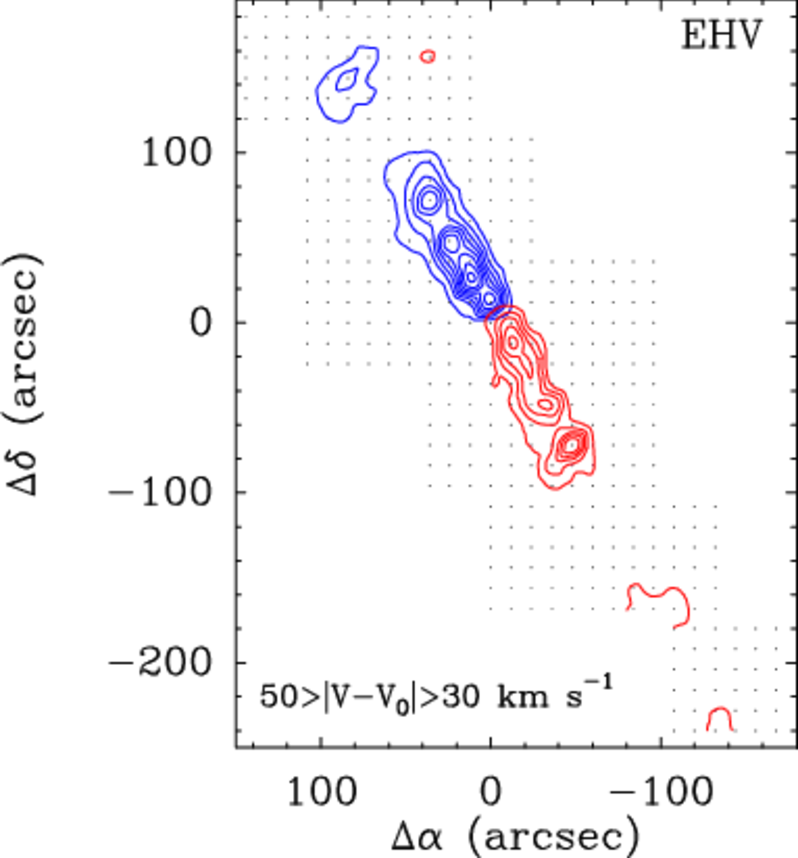
\includegraphics[width=\linewidth]{outflow_tafalla04}
\caption[Outflow in CO($2\rightarrow 1$)]{
\label{fig:outflow_tafalla04}
An integrated intensity map in CO($2\rightarrow 1$), showing material at velocities between $\pm 30-50$ km s$^{-1}$ (\textit{blue and red contours, respectively}) relative to the mean \citep{tafalla04c}. Contours are spaced at intensities of 1 K km s$^{-1}$. The outflow shown is in the Taurus star-forming region.
}
\end{marginfigure}

However, there might be other indicators that a star has formed. For example, the density distribution might show a very sharp, unresolved peak. Another sign that a star has formed might be the presence of an outflow, which, as we discuss in Chapter \ref{ch:disks_obs}, all protostars seem to generate. Outflows coming from the center of a core can be detected in a few ways. Most directly, one can see bipolar, high velocity structures in molecular emission (Figure \ref{fig:outflow_tafalla04}). One can also detect indirect evidence of an outflow, from the presence of highly excited molecular line emission that is produced by shocks at hundreds of km s$^{-1}$. One example of such a line is SiO($2\rightarrow 1)$ line, which is generally seen in gas moving at several tens of km s$^{-1}$ with temperatures of several hundred K -- this is taken to be indication that emission in this line is produced in warm shocks. Since we know of no processes other than formation of a compact object with a $\gtrsim 100$ km s$^{-1}$ escape velocity that can accelerate gas in molecular clouds to such speeds, the presence of such an outflow is taken to indicate that a compact object has formed.

\begin{marginfigure}
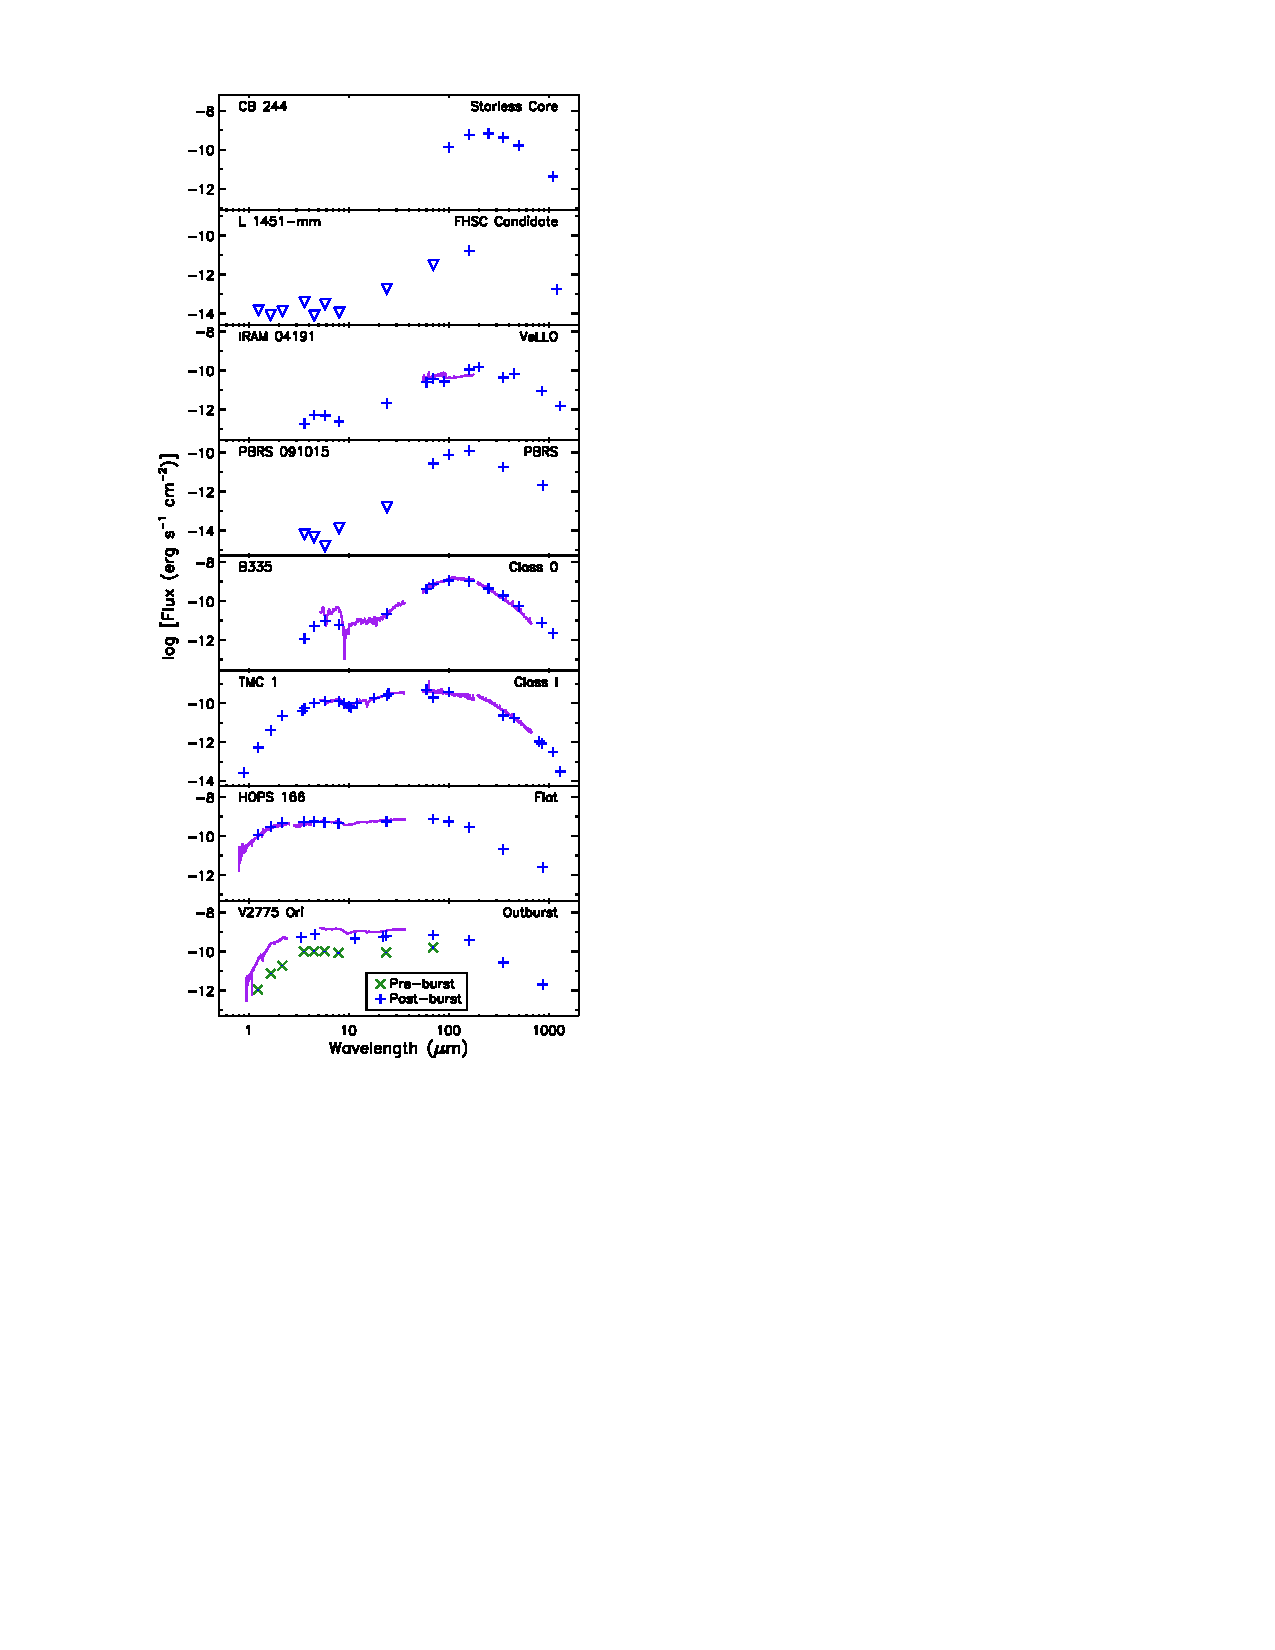
\includegraphics[width=\linewidth]{seds_dunham14}
\caption[Sample SEDs of protostellar cores]{
\label{fig:seds_dunham14}
Sample spectral energy distributions (SEDs) of protostellar cores, together with the assigned class, as collected by \citet{dunham14a}.
}
\end{marginfigure}

These are the earliest indications of star formation we have available to us. We call objects that show one of these signs, and do not fall into one of the other categories, class 0 sources. The dividing line between class 0 and class 1 is that the star begins to heat the dust around it to the point that there is non-trivial infrared emission. Before the advent of \textit{Spitzer} and \textit{Herschel}, the dividing line between class 0 and 1 was taken to be a non-detection in the IR, but as more sensitive IR telescopes became available, the detection limit went down, and it became necessary to specify a dividing line in terms of a luminosity cut. A source is said to be class 0 if more than 0.5\% of its total bolometric output emerges at wavelengths longer than $350$ $\mu$m, i.e., if $L_{\rm smm} / L_{\rm bol} > 0.5\%$, where $L_{\rm smm}$ is defined as the luminosity considering only wavelengths of 350 $\mu$m and longer (Figure \ref{fig:seds_dunham14}).

In practice, measuring $L_{\rm smm}$ can be tricky because it can be hard to get absolute luminosities (as opposed to relative ones) correct in the sub-mm, so it is also common to define the class 0-1 divide in terms of another quantity: the bolometric temperature $T_{\rm bol}$. This is defined as the temperature of a blackbody that has the same flux-weighted mean frequency as the observed spectral energy distribution (SED). That is, if $F_\nu$ is the flux as a function of frequency from the observed source, then we define $T_{\rm bol}$ by the implicit equation
\begin{equation}
\frac{\int \nu B_{\nu}(T_{\rm bol}) \, d\nu}{\int B_{\nu}(T_{\rm bol}) \, d\nu} = \frac{\int \nu F_{\nu}\, d\nu}{\int F_\nu \,d\nu}.
\end{equation}
The class 0-1 dividing line is also sometimes taken to be $T_{\rm bol} = 70$ K. In cases where $L_{\rm smm}$ is accurately measured, $T_{\rm bol}$ is observed to be a reasonably good proxy for $L_{\rm smm} / L_{\rm bol}$ (Figure \ref{fig:tbol_dunham14}).

\begin{marginfigure}
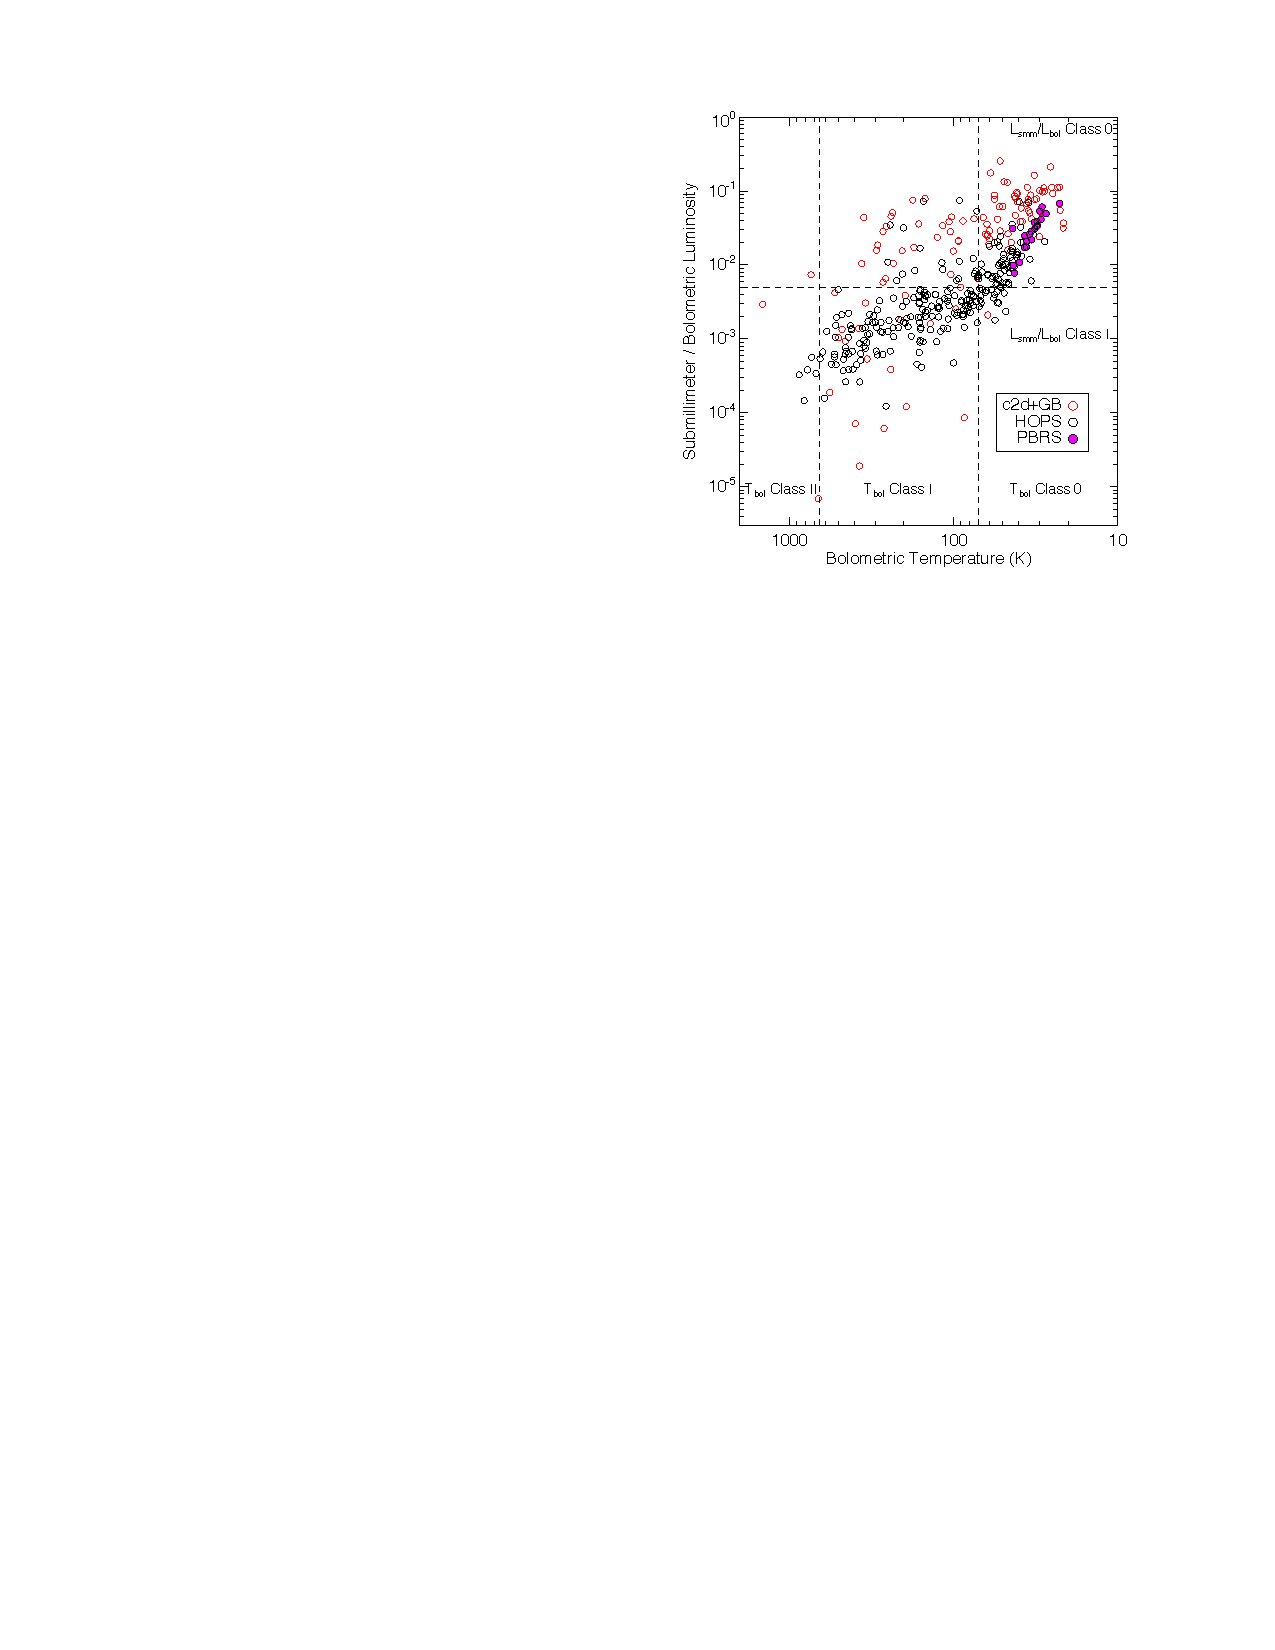
\includegraphics[width=\linewidth]{tbol_dunham14}
\caption[Bolometric temperatures of protostellar cores]{
\label{fig:tbol_dunham14}
Bolometric temperatures of protostellar cores as compared to sub-mm to bolometric luminosity ratios \citep{dunham14a}. The samples shown are from three different surveys as indicated in the legend.
}
\end{marginfigure}

Once protostars reach class I, their evolution into further classes is defined in terms of the infrared spectral energy distribution. The motivating cartoon is a follows. At early times, the envelope of dust around the protostar is very optically thick at visible and even near infrared wavelengths. As a result, we cannot directly observe the stellar photosphere. All the radiation is absorbed by the envelope. The dust is in thermal equilibrium, so it re-radiates that energy. Since the radius of the sphere of dust is much larger than that of the star, and the luminosity radiated by the dust must ultimately be equal to that of the star, this emission must be at lower temperature and thus longer wavelengths. Thus as the radiation propagates outward through the dust it is shifted to longer and longer wavelengths. However, at wavelengths longer than the characteristic sizes of the dust grains, the opacity decreases as roughly $\kappa_\lambda \propto \lambda^{-2}$. Thus eventually the radiation is shifted to wavelengths where the remaining dust is optically thin, and it escapes. What we observe is therefore not a stellar photosphere, but a "dust photosphere".

Given this picture, the greater the column density of the dust around the star, the further it will have to diffuse in wavelength in order to escape. Thus the wavelength at which the emission peaks, or, roughly equivalently, the slope of the spectrum at a fixed wavelength, is a good diagnostic for the amount of circumstellar dust. Objects whose SEDs peak closer to the visible are presumed to be more evolved, because they have lost more of their envelopes.

More formally, this classification scheme was based on fluxes as measured by the \textit{Infrared Astronomical Satellite (IRAS)}. We define
\begin{equation}
\alpha_{\rm IR} = \frac{d\log (\lambda F_{\lambda})}{d\log\lambda},
\end{equation}
as the infrared spectral index, and in practice we measure $\alpha_{\rm IR}$ using two points from the \textit{IRAS} SED: 2.2 $\mu$m and $10-25$ $\mu$m. More positive values of $\alpha_{\rm IR}$ indicate SEDs that peak at longer wavelengths, further into the IR, while more negative values indicate SEDs that peak closer to visible. We define sources with $\alpha_{\rm IR}\geq 0.0$, i.e., rising at longer wavelengths from 2 to 25 $\mu$m, as class I sources. Alternately, in terms of bolometric temperature, the class I to class II transition is generally taken to be at 650 K (Figure \ref{fig:seds_dunham14}).

As more of the envelope accretes, it eventually becomes optically thin at the peak emitting wavelengths of the stellar photosphere. In this case we see the stellar blackbody spectrum, but there is also excess infrared emission coming from the disk of warm, dusty gas that still surrounds the star. Thus the SED looks like a stellar blackbody plus some extra emission at near- or mid-infrared wavelengths. Stars in this class are also know as classical T Tauri stars, named for the first object of the class, although the observational definition of a T Tauri star is somewhat different than the IR classification scheme\footnote{T Tauri stars were first identified in the optical, long before the availability of infrared SEDs. They are defined by high levels of optical variability and the presence of strong chromospheric lines, indicating large amounts of circumstellar material. T Tauri stars are discussed further in Chapter \ref{ch:late_disk}.}, so the alignment may not be perfect. In terms of $\alpha_{\rm IR}$, these stars have indices in the range $-1.6 < \alpha_{\rm IR} < 0$.\footnote{Depending on the author, the breakpoint may  be placed at $-1.5$ instead of $-1.6$. Some authors also introduce an intermediate classification between 0 and I, called flat spectrum sources, which they take to be $-0.3 < \alpha_{\rm IR} < 0.3$.} A slope of around $-1.6$ is what we expect for a bare stellar photosphere without any excess infrared emission coming from circumstellar material. Since the class II phase is the last one during which there is a disk of any significant mass, this is also presumably the phase where planet formation must occur.

The final stages is class III, the category into which we places sources whose SEDs have $\alpha_{\rm IR} < -1.6$. Stars in this class correspond to weak line T Tauri stars. The SEDs of these stars look like bare stellar photospheres in the optical through the mid-infrared. If there is any IR excess at all, it is in the very far IR, indicating that the emitting circumstellar material is cool and located far from the star. The idea here is that the disk around them has begun to dissipate, and is either now optically thin at IR wavelengths or completely dissipated, so there is no strong IR excess. 

However, these stars are still not mature main sequence stars. First of all, their temperatures and luminosities do not correspond to those of main sequence stars. Instead, they are still puffed up to larger radii, so they tend to have either lower effective temperatures or higher bolometric luminosities (or both) than main sequence stars of the same mass. Second, they show extremely high levels of magnetic activity compared to main sequence stars, producing high levels of X-ray emission. Third, they show lithium absorption lines in their atmospheres. This is significant because lithium is easily destroyed by nuclear reactions at high temperatures, and no main sequence stars with convective photospheres show Li absorption. Young stars show it only because there has not yet been time for all the Li to burn.

\section{Statistics of Resolved Stellar Populations}

Young stars tend to be born in the presence of other stars, rather than by themselves. This is not surprising: the gas cores from which they form are very small fragments, $\sim 1$ $\msun$, inside much larger, $\sim 10^6$ $\msun$ clouds. It would be surprising if only one tiny fragment containing $\sim 10^{-6}$ of the total cloud mass were to collapse. We now pull back to somewhat larger scales to look at the formation of stars in groups.

\subsection{Multiplicity}

The smallest scale we can look at beyond a single star is multiple systems. When we do so, we find that a significant fraction of stars are members of multiple systems -- usually binaries, but also some triples, quadruples, and larger. The multiplicity is a strong function of stellar mass. The vast majority of B and earlier stars are multiples, while the majority of G, K, and M stars are singles. This means that most stars are single, but that most massive stars are multiples. The distribution of binary periods is extremely broad, ranging from hours to Myr. The origin of the distribution of periods, and of the mass-dependence of the multiplicity fraction, is a significant area of research in star formation theory, one to which we will return in Chapters \ref{ch:imf_obs}, \ref{ch:imf_th}, and \ref{ch:massivestar}.

\subsection{The Initial Mass Function}

If we observe a cluster of stars, the simplest thing to do is simply count up how many of them there are as a function of mass. The result is one of the most important objects in astrophysics, the initial mass function (IMF). This requires a bit of modeling, since of course what we can actually measure is a luminosity function, not a mass function. The problem of determining the IMF can be tackled in two ways: either by looking at stars in the solar neighborhood, or by looking at individual star clusters.

Looking at stars in the Solar neighborhood has the advantage that there are a lot of them compared to what you see in a clusters, so one gets a lot of statistical power. One also does not have to worry about two things that a major headache for studies of young clusters. First, young clusters usually have remaining bits of gas and dust around them, and this creates reddening that can vary with position and has to be modeled. Second, for clusters younger than $\sim 10$ Myr, the stars are not on the main sequence yet. Since young stars are brighter than main sequence stars of the same mass, this produces and age-mass degeneracy that you have to break by obtaining more information that just luminosities (usually temperatures or colors), and then making pre-main sequence evolutionary models.\footnote{Protostellar evolution is covered in Chapter \ref{ch:protostar_evol}.}

On the other hand, if we want to talk about the IMF of massive stars, we are largely stuck looking at young clusters. The same is also true for brown dwarfs. Since these fade with time, it is hard to find a large number of them outside of young clusters. An additional advantage of star clusters is that they are to good approximation chemically homogenous, so we need not worry about chemical variations masquerading as mass variations.

A big problem for either method is correction for unresolved binaries, particularly at the low mass end, where the companions of brighter stars are very hard to see. When one does all this, the result is the apparently universal or close-to-universal distribution illustrated in Figure \ref{fig:imf_bastian10}.\footnote{There have been recent claims of IMF variation from extragalactic observation, which we will discuss in Chapter \ref{ch:imf_obs}.} The basic features we see are a break peak centered around a few tenths of $\msun$, with a fairly steep fall off at higher masses that is well fit by a powerlaw function with a slope near $-2.3$. There is also a fall-off at lower masses, although some authors argue for a second peak in the brown dwarf regime. This is a difficult observational problem, both because brown dwarfs are hard to find, and because their evolutionary tracks are less secure than those for more massive stars.

\begin{figure}
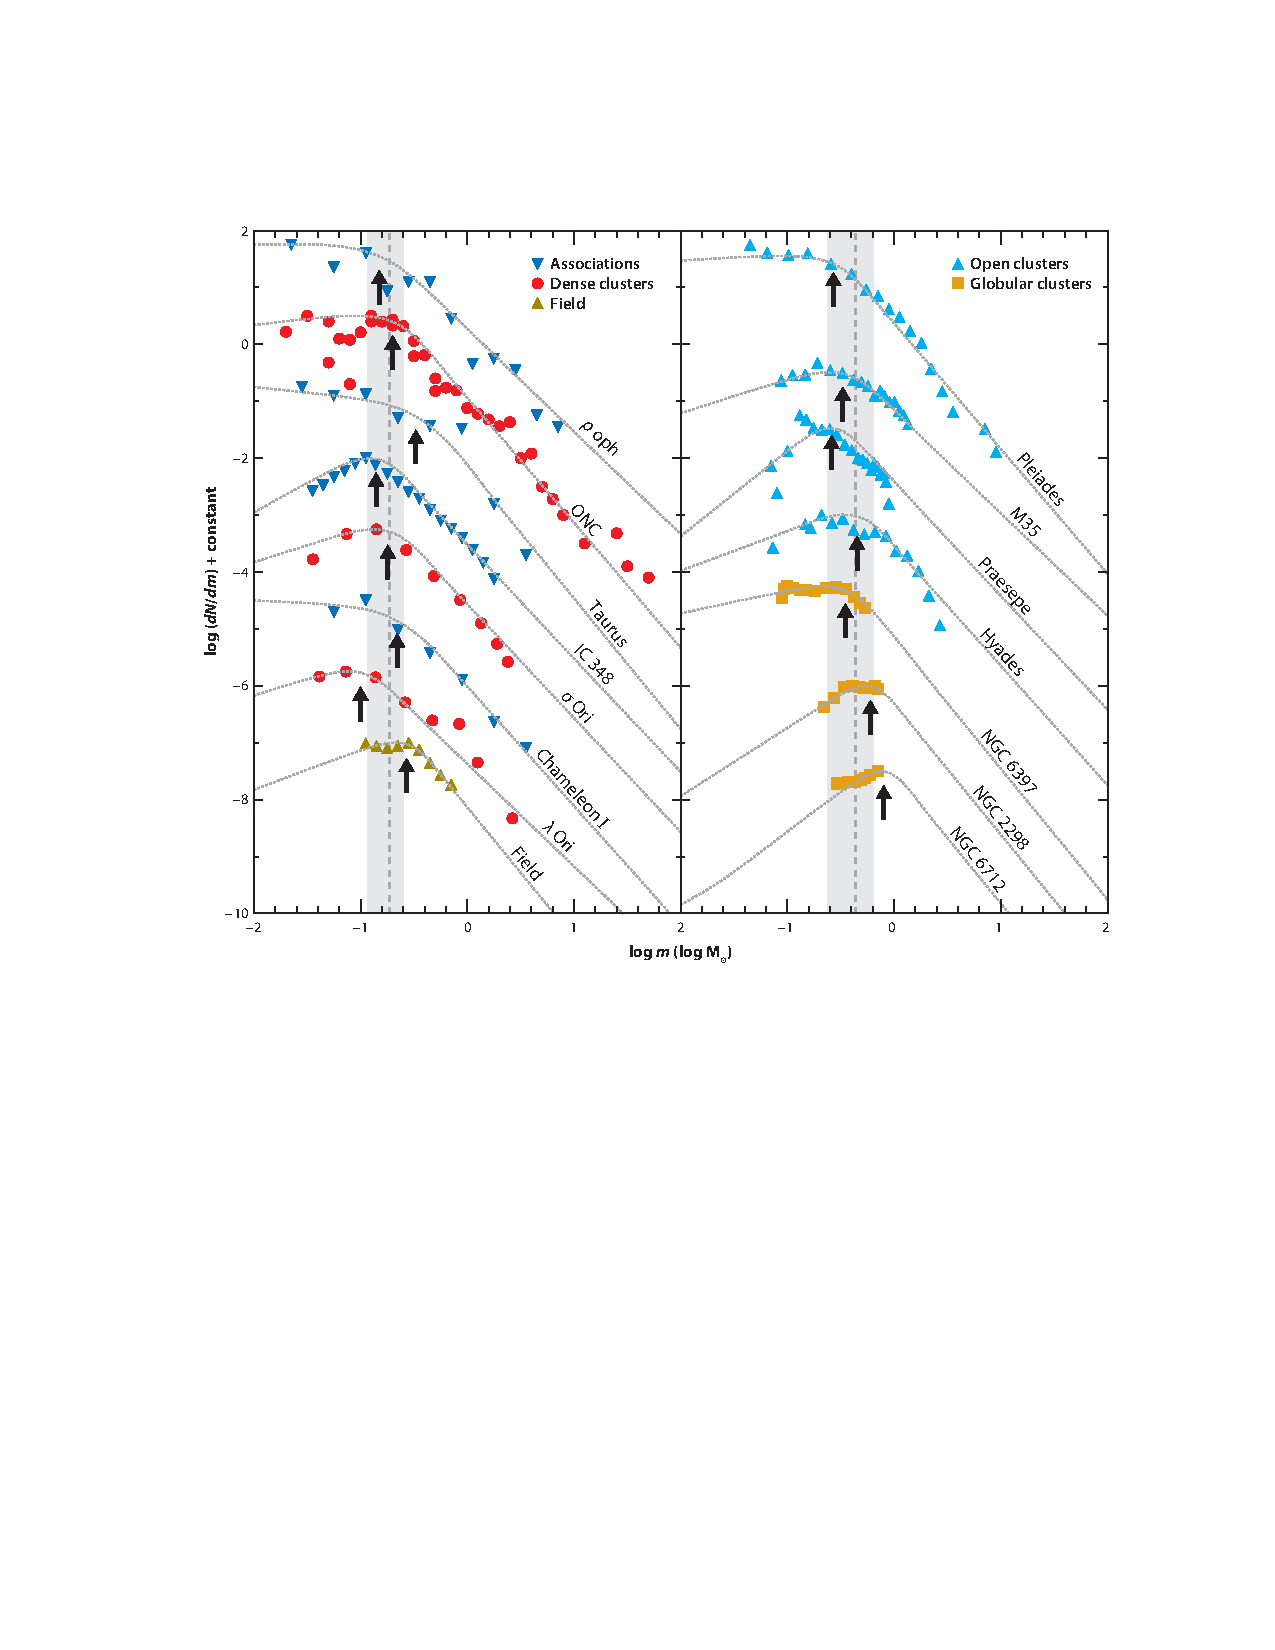
\includegraphics[width=\linewidth]{imf_bastian10}
\caption[Measured stellar IMFs in a variety of regions]{
\label{fig:imf_bastian10}
Stellar initial mass functions inferred for a wide variety of regions in the Milky Way, with the type of region as indicated in the legend \citep{basian10a}. The dashed lines represents powerlaw fits to the observations in each region, with the black arrows indicating the best fit turnover mass.
}
\end{figure}

The functional form shown in Figure \ref{fig:imf_bastian10} has been parameterized in a number of ways. Two of the most popular are from \citet{kroupa01a, kroupa02c} and \citet{chabrier03a, chabrier05a}.\footnote{See the reviews by \citet{bastian10a} and \citet{offner14a} for a thorough listing of alternate parameterizations.}  Both of these fit the field star data, and the data individual clusters, within the error bars. The functional form for Chabrier is
\begin{equation}
\label{eq:chabrier}
\frac{dn}{d\log m} \propto 
\left\{
\begin{array}{ll}
\exp\left[-\frac{(\log m-\log 0.22)^2}{2\times 0.57^2}\right], &
m<1 \\
\exp\left[-\frac{(-\log 0.22)^2}{2\times 0.57^2}\right] m^{-1.35}, &
m\ge 1
\end{array}
\right.,
\end{equation}
while the functional form for Kroupa is
\begin{equation}
\label{eq:kroupa}
\frac{dn}{d\log m} \propto
\left\{
\begin{array}{ll}
\left(\frac{m}{m_0}\right)^{-\alpha_0}, & m_0 < m < m_1\\
\left(\frac{m_1}{m_0}\right)^{-\alpha_0} \left(\frac{m}{m_1}\right)^{-\alpha_1}, &
m_1 < m < m_2 \\
\left[\prod_{i=1}{n} \left(\frac{m_i}{m_{i-1}}\right)^{-\alpha_i}\right] \left(\frac{m}{m_n}\right)^{-\alpha_n}, &
m_{n-1} < m < m_n
\end{array}
\right.,
\end{equation}
with
\begin{equation}
\begin{array}{ll}
\alpha_0 = -0.7\pm 0.7, & m_0 = 0.01 \\
\alpha_1 = 0.3\pm 0.5, & m_1 = 0.08 \\
\alpha_2 = 1.3\pm 0.3, & m_2 = 0.5 \\
\alpha_3 = 1.3\pm 0.7, & m_3 = 1 \\
\end{array}.
\end{equation}
In both of the above expressions, $m$ is understood to be in units of $M_\odot$.

\section{Unresolved Stellar Populations and Extragalactic Star Formation}

What about cases where we cannot resolve the stellar population, as is usually the case for extragalactic work? What can we learn about star formation in that case? The answer turns out to be that the thing we can most directly measure is the star formation rate, and that doing so yields some very interesting results.

\subsection{Measuring the Star Formation Rate: General Theory}

The most basic problem in working with unresolved stellar populations is how we distinguish young stars from main sequence ones. Except for the brightest stars in the nearest galaxies, we cannot obtain spectra, or even colors, for individual stars as we can in the Milky Way. Instead, the strategy we use to isolate young stars is to exploit the fact that massive stars have short lifetimes, so if we measure the total number of massive stars in a galaxy, or some patch of a galaxy, then we are effectively measuring we many such stars formed there over some relatively short period. We can formalize this theory a bit as follows.

Consider stars born with an initial mass function $dn/dm$. The mean stellar mass for this IMF is $\overline{m} = \int dm\, m(dn/dm)$. A time $t$ after a star is born, the star has a luminosity $L(m,t)$, where the luminosity can be bolometric, or integrated over some particular filter or wavelength range. First consider the simplest possible case, a population of stars all born at the same instant at time $0$. A time $t$ later, the luminosity of the stars is
\begin{equation}
L(t) = N_* \int_0^{\infty} dm\, L(m,t) \frac{dn}{dm},
\end{equation}
where $N_*$ is the total number of stars, and we have normalized the IMF so that $\int (dn/dm) \, dm = 1$. That is, we simply integrate the luminosity per star at time $t$ over the mass distribution of stars. Now consider a region, e.g., a galaxy, forming stars at a rate $\dot{M}_*(t)$; in terms of number, the star formation rate is $\dot{N}_*(t) = \dot{M}_*(t)/\overline{m}$. To find the luminosity of the stellar population that is present today, we simply take the expression we just derived and integrate over all the possible stellar ages. Thus we have
\begin{equation}
L =  \int_{0}^\infty dt\, \frac{\dot{M}_*(t)}{\overline{m}}  \int_0^{\infty} dm\, L(m,t) \frac{dn}{dm}.
\end{equation}

By itself this is of limited use, because the right hand side depends on the full star formation history $\dot{M}_*(t)$. However, let us assume that $\dot{M}_*$ is constant in time. The integral still converges as long as $L(m,t)$ reaches 0 after a finite time. In this case the integrals over $m$ and $t$ are separable, and we can rearrange them to
\begin{equation}
\label{eq:sfrtol}
L = \frac{\dot{M}_*}{\overline{m}} \int_0^{\infty} dm \, \frac{dn}{dm} \int_0^\infty dt \, L(m,t) \equiv \frac{\dot{M}_*}{\overline{m}} \int_0^{\infty} dm \, \frac{dn}{dm} \langle L t_{\rm life} \rangle_m 
\end{equation}
In the final step we defined a new quantity $\langle L t_{\rm life} \rangle_m$, which has a simple physical meaning: it is the total amount of radiant energy that a star of mass $m$ puts out over its lifetime.

Notice the expression on the right depends only on the constant star formation rate $\dot{M}_*$, the energy output $\langle L t_{\rm life}\rangle_m$, which we can generally calculate from stellar structure and evolution theory, and the IMF $dn/dm$. Thus if we measure $L$ and use the "known" values of  $\langle L t_{\rm life}\rangle_m$ and $dn/dm$, we can measure the star formation rate. The underlying physical assumption is that the stellar population being observed is in statistical equilibrium between new stars forming and old stars dying, so the total number of stars present and contributing to the light at any time is proportional to the rate at which they are forming. Thus a measurement of the light tells us about the star formation rate.

Is our assumption that $\dot{M}_*$ is constant reasonable? That depends on the system we are observing. For an entire galaxy that is forming stars quiescently and has not been externally perturbed, it is probably reasonable to assume that $\dot{M}_*$ cannot vary on timescales much shorter than the dynamical time of the galaxy, which is $\sim 200$ Myr for a galaxy like the Milky Way. If we choose to observe the luminosity at a wavelength where the light is coming mostly from stars with lifetimes shorter than this, so that $L(m,t)$ reaches 0 (at least to good approximation) at times much less than 200 Myr, then assuming constant $\dot{M}_*$ is quite reasonable.

However, it is always important to keep this constraint in mind -- we can only measure the star formation rate as long as we believe it to be constant on timescales long compared to the lifetimes of the stars responsible for generating the luminosity we are measuring. One can actually see how the ratio of luminosity to star formation rate behaves in systems that do not satisfy the constraint by generating synthetic stellar populations. In the simple case of a system that begins with no stars and then forms star stars at a constant rate, the bolometric luminosity after the onset of star formation just increases linearly with time until the first stars star evolving off the main sequence, and only becomes constant after $\sim 4$ Myr (Figure \ref{fig:lvst_krumholz07}).

\begin{marginfigure}
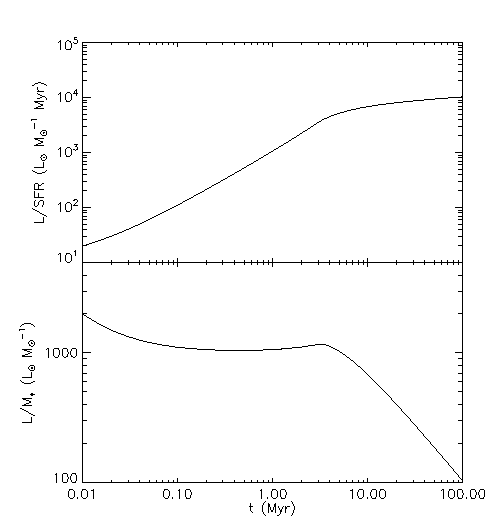
\includegraphics[width=\linewidth]{lvst_krumholz07}
\caption[Bolometric luminosity versus stellar population age]{
\label{fig:lvst_krumholz07}
Bolometric luminosity versus time for stellar populations as a function of population age. The top panel shows the luminosity normalized by the star formation rate, while the bottom shows the luminosity normalized by the total stellar mass. Figure taken from \citet{krumholz07e}.
}
\end{marginfigure}

The need to satisfy this constraint generally drives us to look for luminosities that are dominated by very massive stars, because these have very short lifetimes. Thus we will begin by discussing what luminosities we can measure that are particularly good at picking out massive stars. This is far from an exhaustive list -- astronomers have invented many, many methods to infer star formation rates for galaxies at a range of redshifts. The accuracy of these techniques is highly variable, and in some cases amounts to little more than a purely empirical calibration. We focus here on the most reliable and widely used techniques that we can apply to relatively nearby galaxies.

\subsection{Recombination Lines}

Probably the most common technique, and the only one that can be used from the ground for most galaxies, is hydrogen recombination lines. To illustrate why this is useful, it is helpful to look at some galaxy spectra (Figure \ref{fig:spectra_kennicutt92}). As we move from quiescent E4 and SB galaxies to actively star-forming Sc and Sm/Im galaxies, there is a striking different in the prominence of emission lines.

\begin{figure}
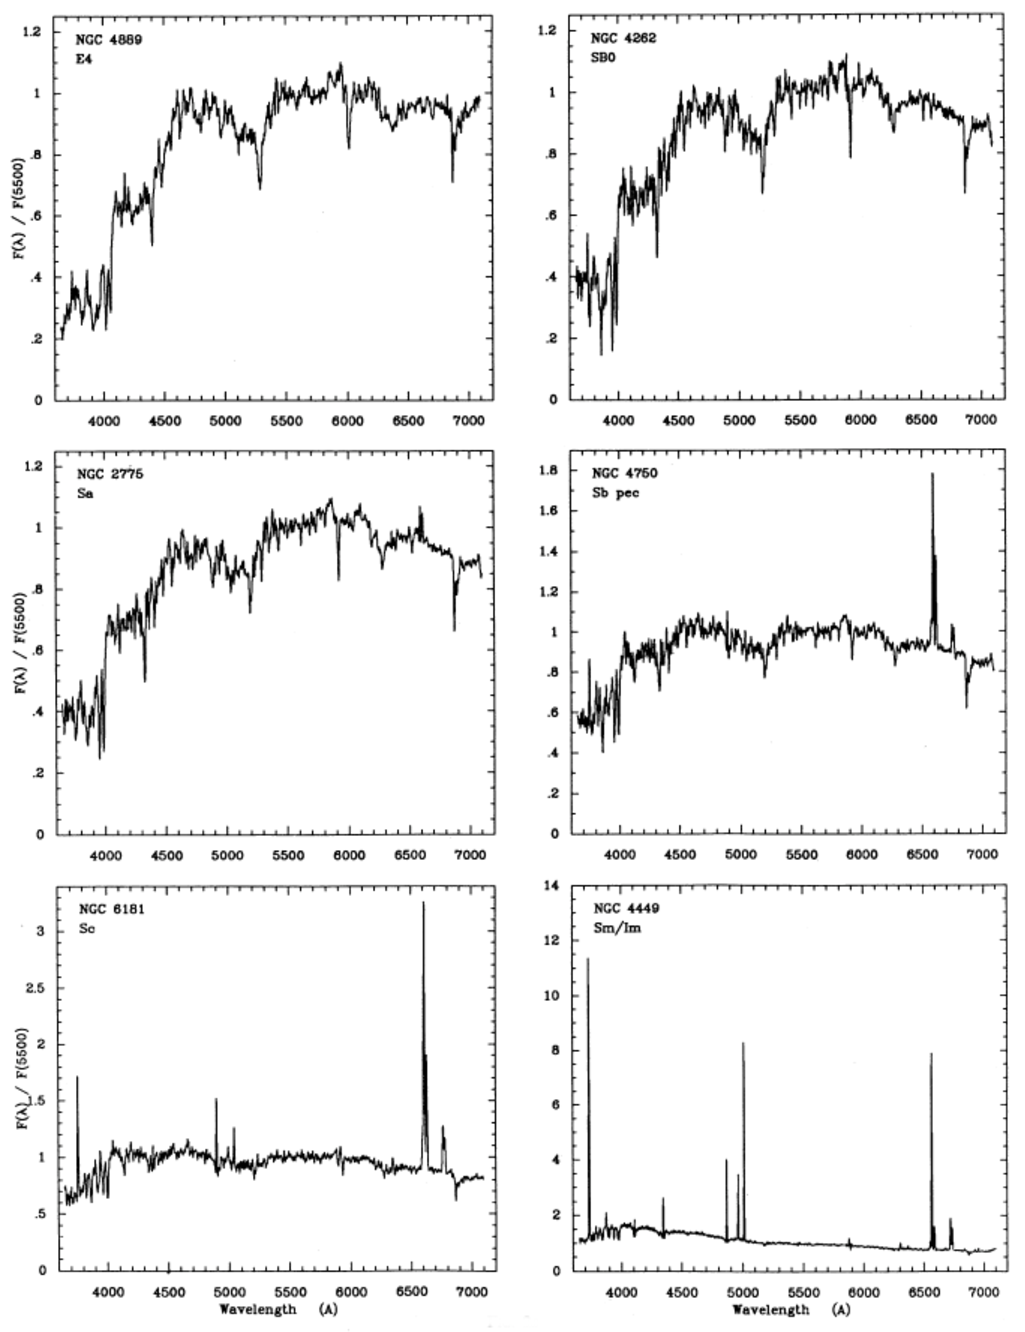
\includegraphics[width=\linewidth]{spectra_kennicutt92}
\caption[Optical spectra of galaxies across the Hubble sequence]{
\label{fig:spectra_kennicutt92}
Example spectra of galaxies of varying Hubble type, from the atlas of \citet{kennicutt92a}. In each panel, the galaxy name and Hubble type are listed.
}
\end{figure}

In the example optical spectra, the most prominent lines are the H$\alpha$ line at 6563 \AA\ and the H$\beta$ at 4861 \AA. These are lines produced by the $3\rightarrow 2$ and $4\rightarrow 2$, respectively, electronic transitions in hydrogen atoms. In the infrared (not shown in the figure) are the Paschen $\alpha$ and $\beta$ lines at 1.87 and 1.28 $\mu$m, and the Bracket $\alpha$ and $\gamma$ lines at 4.05 and 2.17 $\mu$m. These come from the $4\rightarrow 3$, $5\rightarrow 3$, $5\rightarrow 4$, and $7\rightarrow 4$ transitions.

Why are these related to star formation? The reason is that these lines come from H~\textsc{ii} regions: regions of ionized gas produced primarily by the ionizing radiation of young stars. Since only massive stars (lager than $10-20$ $\msun$) produce significant ionizing fluxes, these lines indicate the presence of young stars. Within these ionized regions, one gets hydrogen line emission because atoms sometimes recombine to excited states rather than to the ground state. These excited atoms then radiatively decay down to the ground state, producing line emission in the process.

Obtaining a numerical conversion between the observed luminosity in one of these lines and the star formation rate is a four-step process. First, one performs a quantum statistical mechanics calculation to compute the yield of photons in the various lines per recombination. This can be done very precisely from first principles. Second, one equates the total recombination rate to the total ionization rate, and uses this to determine the total rate of emission for the line in question per ionizing photon injected into the nebula. Third, one uses stellar models to compute $\langle L_{\rm ion} t_{\rm life}\rangle_m$, the total ionizing photon production by a star of mass $m$ over its lifetime. Four, one evaluates the integral over the IMF given by equation (\ref{eq:sfrtol}) to obtain the numerical conversion between star formation rate and luminosity. As of this writing, the most up-to-date resource for the results of such calculations is \citet{kennicutt12a}.

Note that there are significant uncertainties in these numbers, the dominant one of which is the IMF. The reason the IMF matters so much is that the light is completely dominated by the massive stars, while the mass is all in the low mass stars that are not observed directly. To give an example, for a Chabrier IMF at zero age, stars more massive than 15 $\msun$ contribute 99\% of the total ionizing flux for a stellar population, but constitute less than 0.3\% of the mass. Thus we are extrapolating by at least a factor of 30 in mass, and small changes in the IMF can produce large changes in the resulting ionizing luminosity to mass conversion.

Another complication is that some of the line emission is likely to be absorbed by dust grains within the source galaxy, and some of the ionizing photons are absorbed by dust grains rather than hydrogen atoms. Thus, one must make an extinction correction to the luminosities.

\subsection{Radio Free-Free}

A closely related method for measuring massive stars is to use free-free emission at radio wavelengths. An H~\textsc{ii} region emits optical lines from transitions between energy levels of hydrogen and other atoms, but it also emits free-free radiation in the radio. This is radiation produced by bremsstrahlung: free electrons scattering off ions, and emitting because accelerating charges emit. It is the opposite side of the coin from recombination line emission: the former occurs when free electrons and protons encounter one another and do not become bound, while the latter occurs when they do.

We will not treat bremsstrahlung or its application to H~\textsc{ii} regions here, but the relevant point for us is that the free-free luminosity of H~\textsc{ii} regions at radio wavelengths is proportional to $n_e n_i$, i.e., the product of the electron and ion densities. Since the recombination rate is also proportional to $n_e n_{\rm H^+}$, and due to chemical balance the recombination rate must equal the ionization rate, the free-free luminosity is directly proportional to the rate at which ionizing photons are injected into the H~\textsc{ii} region. Thus one can convert between free-free emission rate and ionization rate based on the physics of H~\textsc{ii} regions, and from then convert that into a star formation rate exactly as for optical recombination lines.

The free-free method has one major advantage, which is that radio emission is not obscured by dust, so one of the dust absorption corrections goes away. The correction for absorption of ionizing photons by dust grains within the H~\textsc{ii} region remains, but this is generally only a few tens of percent. Thus radio free-free measurements are more reliable that recombination line ones. Indeed, they are the only technique we can use for most H~\textsc{ii} regions in the Milky Way, since these tend to be located in the Galactic plane and thus suffer from heavy extinction at optical wavelengths. The downside is that the free-free emission is quite weak, and separating free-free from other sources of radio emission requires the ability to resolve individual H~\textsc{ii} regions. Thus at present this technique is useful primarily for the Milky Way and a few other nearby galaxies, since those are the only places where we can detect and resolve individual H~\textsc{ii} regions.

\subsection{Infrared}

The recombination line methods work well for galaxies that are like the Milky Way, but considerably less well for galaxies that are dustier and have higher star formation rates. This is because the dust extinction problem becomes severe, so that the vast majority of the Balmer line emission is absorbed. The Paschen and Bracket emission is much less sensitive to this, since those lines are in the IR, but even they can be extincted in very dusty galaxies, and they are also much harder to use than H$\alpha$ and H$\beta$ because they are $1-2$ orders of magnitude less bright intrinsically.

Instead, for dusty sources the tracer of choice is far infrared. The idea here is that, in a sufficiently dusty galaxy, essentially all stellar light will eventually be absorbed by dust grains. These grains will then re-emit the light in the infrared. As a result, the SED peaks in the IR. In this case one can simply use the total IR output of the galaxy as a sort of calorimeter, measuring the total bolometric power of the stars in that galaxy. In galaxies or regions of galaxies with high star formation rates, which tend to be where H$\alpha$ and other recombination line techniques fail, this bolometric power tends to be completely dominated by young stars. Since these stars die quickly, the total number present at any given time is simply proportional to the star formation rate.

The derivation of the conversion in this case is very straightforward -- the $L(m,t)$ that is required is just the total bolometeric output of the stars. Results are given in \citet{kennicutt12a}, and Problem Set 1 includes an example calculation. Of course IR emission has its its problems too. First of all, it misses all the optical and UV radiation from young stars that is not absorbed within the galaxy, which makes it a poor choice for dust-poor galaxies where a majority of the radiation from young stars escapes.

A second problem is that if the SFR is low, then old rather than young stars may dominate the bolometric output. In this case the IR indicator can give an artificially high SFR. A more common problem for the dusty galaxies where IR tends to be used most is contamination from an active galactic nucleus (AGN). If an AGN contributes significantly to the bolometric output of a galaxy, that can masquerade as star formation. This can be hard to detect in a very dusty galaxy where most of the AGN light, along with most of the starlight, is absorbed and reprocessed by dust.

\subsection{Ultraviolet}

Yet another way of measuring star formation rates is by the broadband ultraviolet (UV) flux at wavelengths that are longer than 912 \AA\ (corresponding to 13.6 eV, the energy required to ionized hydrogen) but shorter than where old stars put out most of their light. This range is roughly $1250-2500$ \AA. This light does not ionize hydrogen, so unlike shorter wavelengths it can get out of a galaxy.

For galaxies in the right redshift range this light gets redshifted into the visible, so we can see it from the ground. However, for local galaxies these wavelengths are only accessible from space (or least a balloon or rocket). For this reason this band was not used much until the launch of the \textit{Galaxy Evolution Explorer (GALEX)} satellite, which had detectors operating at 1300-1800 and 1800-2800 \AA (referred to as FUV and NUV, respectively). Emission in the FUV band is dominated by stars with masses $\sim 5$ $\msun$ and up, which have lifetimes of $\sim 50$ Myr, so the total FUV light measures the star formation rate integrated over this time scale. Sadly, \textit{GALEX} is no longer in operation, and there is no comparable mission on the immediate horizon, so this technique is largely of archival value for now.

FUV suffers from the same problems with dust extinction as H$\alpha$, and they are perhaps even more severe, since opacity increases as frequency does. On the other hand, FUV is less sensitive to the IMF than H$\alpha$, because ionizing photons come from hotter and thus more massive stars than FUV ones. For systems with low overall star formation rates, ionization-based star formation rate indicators can become quite noisy due to the rarity of the massive stars they trace. FUV has fewer problems in this regard. However, there is a corresponding disadvantage, in that the $\sim 50$ Myr lifetime of FUV-emitting stars is getting uncomfortably close to the typical orbital periods of galaxies, and so one can legitimately worry about whether the SFR has really be constant over the required timescale. This problem becomes even worse if one looks at small-subregions of galaxies, rather than galaxies as a whole. One also has to worry about stars moving from their birth locations over such long timescales.


\subsection{Combined Estimators}

As one might guess from the discussion thus far, none of the indicators by itself is particularly good. Recombination lines and UV get into trouble in dusty galaxies because they miss light from young stars that is obscured by dust, while IR gets into trouble because it misses light from young stars that is not dust-obscured. This suggests that the best way to proceed is to combine one or more estimators, and this is indeed the current state of the art. A number of combined indicators are suggested in \citet{kennicutt12a}.



